\section*{User Interface}

\begingroup
\setlength{\columnsep}{16pt}

\begin{wrapfigure}{r}{4in}
\vspace{-0.3in}
\begin{center}
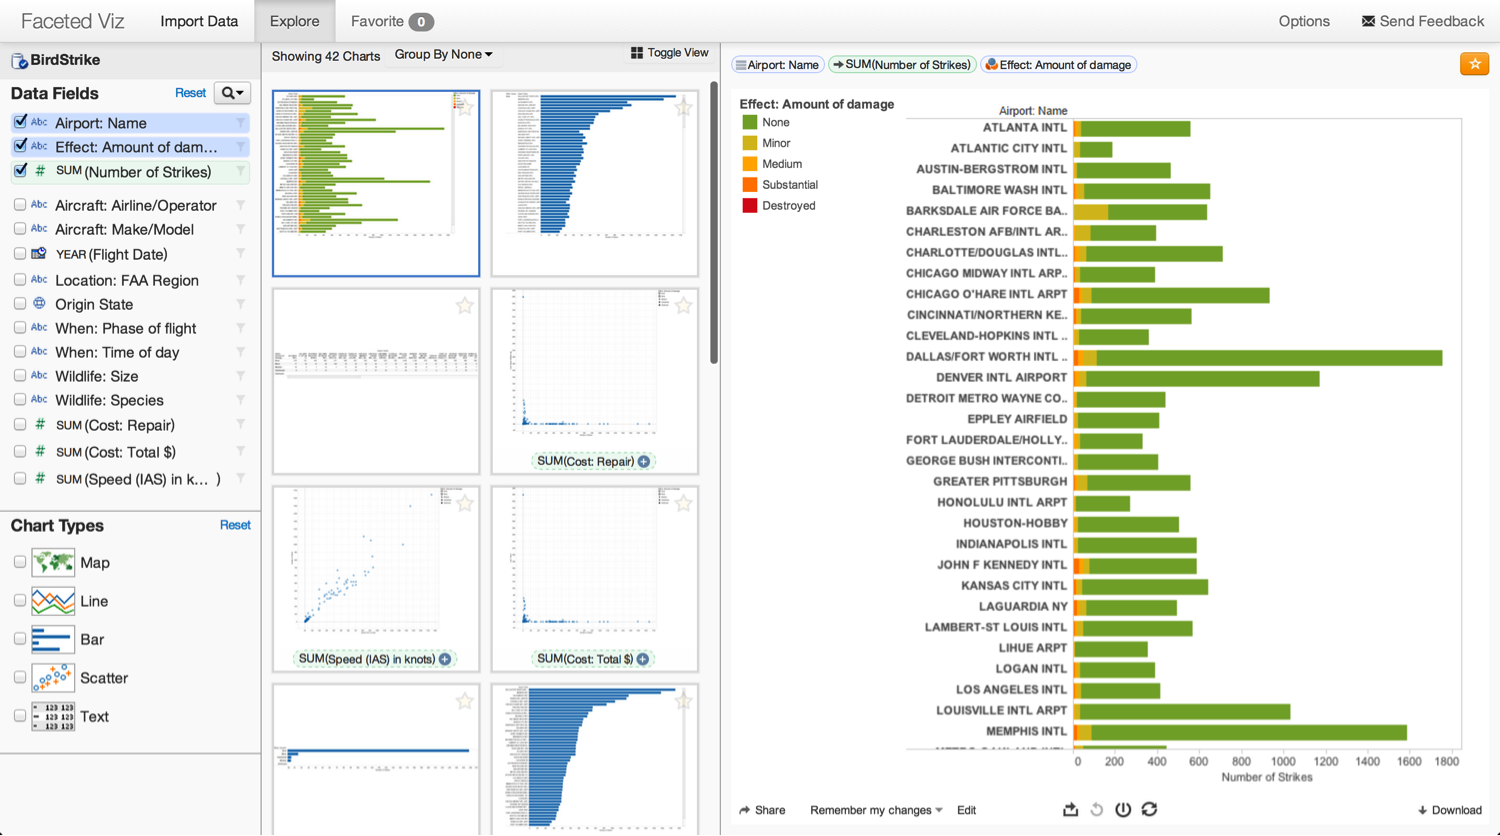
\includegraphics[width=4in]{ui.png}

\caption{Mock-up of our interface. Users can specify their query using controls on the left side.  The browser in the middle displays recommended visualizations.  The interactive view on the right shows the selected visualization.}
\label{fig:ui}
\end{center}
\vspace{-0.3in}
\end{wrapfigure}

Our system will help users focus on data exploration rather than design details by letting users search for visualizations. 
Figure \ref{fig:ui} shows a mock-up of our interface. The interface will highlight data attributes and chart types as two main search facets \cite{yee:faceted}. Prior work indicates that people usually begin describing visualizations by specifying these two properties \cite{grammel:novice}.  Users can also specify data transformations and mappings between data attributes and visual variables. The browser view (Fig. \ref{fig:ui}, middle) will show recommended visualizations based on user input.  Users can then select and interact with a visualization of interest on the right side. The interface will also support the iterative nature of visual analysis.  Analysts can keep refining their queries with more specific intents.  Our interface will also provide annotation and provenance tools to support the analysis flow.


\endgroup

We will build an open-source, scalable interactive visualization module for rendering visualizations, taking specifications generated by the recommendation algorithm as inputs. The module will incorporate design practices such as determining the optimal aspect ratio for the chart type and the data \cite{talbot:arc}.  Output views will support user interactions \cite{heer:dynamics} for data exploration such as highlighting, brushing and linking, zooming, and filtering. The views will also allow the recommender to automatically highlight inferred anomalies and trends.